%************************************************
\chapter{Gli Hook}
\label{cap:hook}
%************************************************

Gli Hook sono delle componenti del framework CodeIgniter con cui probabilmente molti di voi non dovranno mai avere niente a che fare: è comunque importante essere consapevoli della loro esistenza. CodeIgnition è molto flessibile e ogni suo aspetto può essere facilmente configurato per adattarsi alle preferenze dello sviluppatore del progetto. Personalizzare però gli elementi core del framework è un lavoro che non dovrebbe mai essere svolto, se non da professionisti, altrimenti il rischio è quello di compromettere le funzionalità del tool di funzioni con conseguente sulla loro stabilità ed efficienza.
 
Nonostante CodeIgniter funzioni in base al diagramma\vref{img:flowchart}, è possibile modificare alcuni operazioni nel normale flusso di esecuzione, come per esempio caricare un particolare script prima che venga eseguito un proprio Controller, oppure subito dopo. Questa operazione si può attuare grazie ad un Hook che permetterà di svolger questo specifico compito in fase di esecuzione senza dover modificare il core di CodeIgniter.

Gli strumenti che CodeIgnition mette a disposizione dello sviluppatore per svolgere queste personalizzazioni avanzate, senza compromettere la stabilità del core, prendono il nome di \var{Hook}.

\begin{figure}
\centering
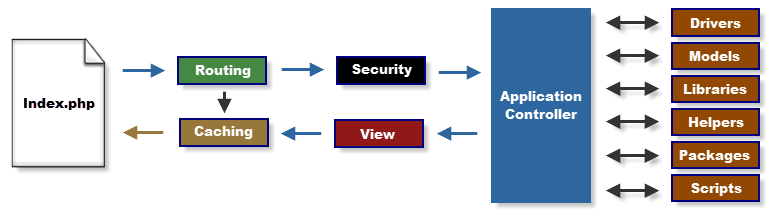
\includegraphics[width=0.7\linewidth]{img/10}
\caption[]{Flow chart}
\label{fig:flowchart}
\end{figure}

Gli Hook si possono abilitare o meno, personalizzando il file \fil{config.php} precedentemente incontrato (si veda sezione\vref{sec:config}), al percorso \sys{application/config/config.php}

Modificando il valore booleano del parametro \verb|$config['enable_hooks']| si potranno abilitare gli Hook (TRUE) o disabilitarli (FALSE). Quest'ultimo è il valore di default.

\section{Utilizzare gli Hook}
La definizione degli Hook è semplice, e avviene agendo sul file \fil{hooks.php} che si trova al percorso \sys{application/config/hooks.php}

La sintassi utilizzata è quella propria di un array in cui è necessario specificare la classe, il metodo, il file, il percorso e gli eventuali parametri. Un esempio chiarificatore è il seguente:

\begin{code}
// Definizione di un Hook
$hook['pre_controller'] = array(
	// nome della classe
    'class'    => 'Classe',

	// nome della funzione di classe
	'function' => 'Funzione',

	// nome del file di classe
	'filename' => 'Classe.php',
	
	// cartella del file di classe
	'filepath' => 'hooks',

	// parametri da elaborare
	'params'   => array('a', 'b', 'c')
);
\end{code}

\section{Definizione di un Hook}
L'Hook viene abilitato agendo su uno specifico array nel percorso \sys{application/config/hooks.php}. Il seguente esempio mostra un prototipo:

\begin{code}
$hook['pre_controller'] = array(

	'class'    => 'MyClass',

	'function' => 'Myfunction',

	'filename' => 'Myclass.php',

	'filepath' => 'hooks',

	'params'   => array('beer', 'wine', 'snacks')

	);
\end{code}
                               
Nota: la parte radice (index) dell'array che nel nostro esempio è \verb|pre_controller|, serve per creare un punto di ancoraggio con l'Hook che si intende utilizzare. Inoltre nell'array sono presente una serie di parametri/indici che devono essere opportunamente configurati:


\begin{description}
\item[class] il nome della classe che si desidera invocare. Se si preferisce usare una funzione procedurale invece di una classe, è necessario lasciare questo campo vuoto.
\item[function] si riferisce al nome della funzione da invocare.
\item[filename] è il nome del file che contiene la classe o funzione.
\item[filepath] si riferisce al nome della directory che contiene il nostro script. Questo deve essere inserito in una directory dentro quella denominata \sys{application/}. Per esempio se lo script si trova \sys{/application/hooks/}, ci si riferirà ad esso semplicemente con \sys{hooks} quando si indicherà il suo percorso. Se invece lo script, sempre facendo un altro esempio, si trova in \sys{/application/hooks/utilities/}, allora il percorso relativo da utilizzare sarà \sys{hooks/utilities} senza lo slash \var{/} iniziale e finale.
\item[params]  ogni parametro, se lo si ritiene necessario, può essere passato al proprio script. Questo parametro è opzionale.
\end{description}

Per un maggiore ordine è vivamente consigliato inserire i propri Hook all'interno di una cartella creata per tale scopo. Se per esempio si volessero inserire i propri script in una cartella chiamata ``mieiscript'', il relativo percorso sarà \sys{application/hooks/Mieiscript} mentre il valore da definire nel \var{filepath} sarà di conseguenza \var{hooks/Mieiscript}.

\section{Gli Hook point}
Gli array in cui sono definiti i parametri descritti prendono il nome di Hook point. Ne esistono diversi, realizzati dagli sviluppatori di CodeIgniter e già pronti all'uso. Quello seguente ne è una parte:

\begin{itemize}
\item \verb|pre_system|: viene chiamato immediatamente dopo la fase di esecuzione, permette unicamente il caricamento delle classi per il benchmark e quelle relative agli Hook stessi;
\item \verb|pre_controller|: ha la massima priorità: viene chiamato precedentemente a qualsiasi Controller; permette il caricamento di classi base come quelle per il routing e la sicurezza
\item \verb|post_controller_constructor|: viene chiamato subito dopo che un Controller è istanziato, ma prima di qualsiasi metodo di classe in esso definito
\item \verb|post_controller|: viene chiamato subito dopo l'esecuzione completa di un Controller;
\item \verb|display_override|: presiede all'override (riscrittura di un metodo ereditato) della funzione \verb|_display()|, utilizzata per inviare gli output al browser web alla fine di un'esecuzione. \'E necessario referenziarsi al super oggetto con \verb|$this->CI =& get_instance()|; i dati finalizzati saranno disponibili attraverso la chiamata \verb|$this->CI->output->get_output()|
\item \verb|cache_override|: consente di utilizzare una propria funzione al posto della funzione di default \verb|_display_cache()| in modo da creare un sistema di cache personalizzato


\item \verb|post_system|: viene chiamato dopo l'invio dell'output al browser al termine di tutte le esecuzioni del sistema
\end{itemize} 

\section{Chiamate multiple allo stesso Hook}

Si può richiamare lo stesso Hook (mediante un punto di ancoraggio) con più di uno script, semplicemente rendendo l'array, con cui facciamo la dichiarazione, multidimensionale; si notino le parentesi quadre dopo le prime in cui viene definito il punto di ancoraggio:

\begin{code}
$hook['pre_controller'][] = array(

	'class'    => 'MyClass',

	'function' => 'Myfunction',

	'filename' => 'Myclass.php',

	'filepath' => 'hooks',

	'params'   => array('birra', 'vino', 'patatine')

	);

$hook['pre_controller'][] = array(

	'class'    => 'MyOtherClass',

	'function' => 'MyOtherfunction',

	'filename' => 'Myotherclass.php',

	'filepath' => 'hooks',

	'params'   => array('rosso', 'giallo', 'blu')

	);
\end{code}


Le seconde parentesi quadre, come nella prima riga \verb|$hook['pre_controller']|\textcolor{red}{[]} permettono di raggiungere lo scopo: definire un array multimensionale per utilizzare il nostro Hook in più script.

\section{Caricamento delle risorse}

CodeIgniter utilizza un sistema di precaricamento che permette alle Librerie, Helper e Modelli di essere inizializzati automaticamente ogni volta che il sistema le richiede. Se invece si ha la necessita che alcune risorse siano sempre disponibili globalmente attraverso la propria applicazione, si dovrà configurare il sistema definito anche come ``auto-load''.

Le seguenti risorse possono essere caricate automaticamente:

\begin{code}
\item le classi core che si trovano nelle directory relative alle Librerie
\item i file Helper che si trovano nelle directory relative agli Helper
\item i file di configurazione che si trovano nella directory config
\item i file del linguaggio che si trovano nella directory system/language/
\item i Modelli che si trovano nelle  directory relative ai Modelli
\end{code}

Per apportare delle modifiche personalizzate è sufficiente agire sul file \fil{autoload.php} al percorso \sys{/application/config/}, semplicemente inserendo le risorse che si desiderano precaricare nell'array. I commenti presenti nel codice dovrebbero essere sufficientemente autoesplicativi.

Nota: come al solito, si ricorda di non inserire l'estensione \var{.php} quando si specifica la risorsa.

\section{Riepilogo}
Gli Hook permettono di intervenire nei meccanismi del funzionamento del framework senza modificarne il core, ovvero il cuore del sistema. Questo permette di creare pericolose instabilità. Ogni sviluppatore può realizzare i propri Hook, definendo delle apposite classi e i relativi metodi, oppure utilizzare quelli predefiniti di CodeIgniter. L'ordine in cui sono richiamati, definisce anche la sequenza di caricamento e di conseguenza la priorità. Infine abbiamo visto che anche se CodeIgniter cerca di caricare le risorse solo quando esse sono necessarie, è possibile ``forzare'' questo comportamento, grazie all'auto-load.